\newpage
\section{Hotspot Analysis}

\subsection{Vectorization}
Questa istruzione non e' vettorizzabile con MSVC, e per tanto, l'esecuzione  risulta essere poco performante.

Mentre con Linux G++, l'operazione sembra ottimizzare \texttt{std::complex}.
\begin{lstlisting}
    z = pow(z, 2) + c;
\end{lstlisting}

\subsection{Hotspot Identification}
The measurements were performed using Intel VTune Profiler and the analysis was performed using Intel Advisor.\\

\begin{center}

    \csvreader[
        tabular= l r r,
        table head=\hline Function Stack & Total & Percentage (\%) \\ \hline,
        late after line=\\,
        late after last line=\\\hline
    ]{assets/hotspots/top-down-tree.csv}{}{%
        \csvcoli & \csvcolii & \csvcoliii
    }
\end{center}

The two main hotspots are the following instructions which takes the most fraction of the program execution.\\

\paragraph{Line 48}
\begin{lstlisting}
    z = pow(z, 2) + c;
\end{lstlisting}

\paragraph{Line 51}
\begin{lstlisting}
    if (abs(z) >= 2)
\end{lstlisting}




\begin{center}
    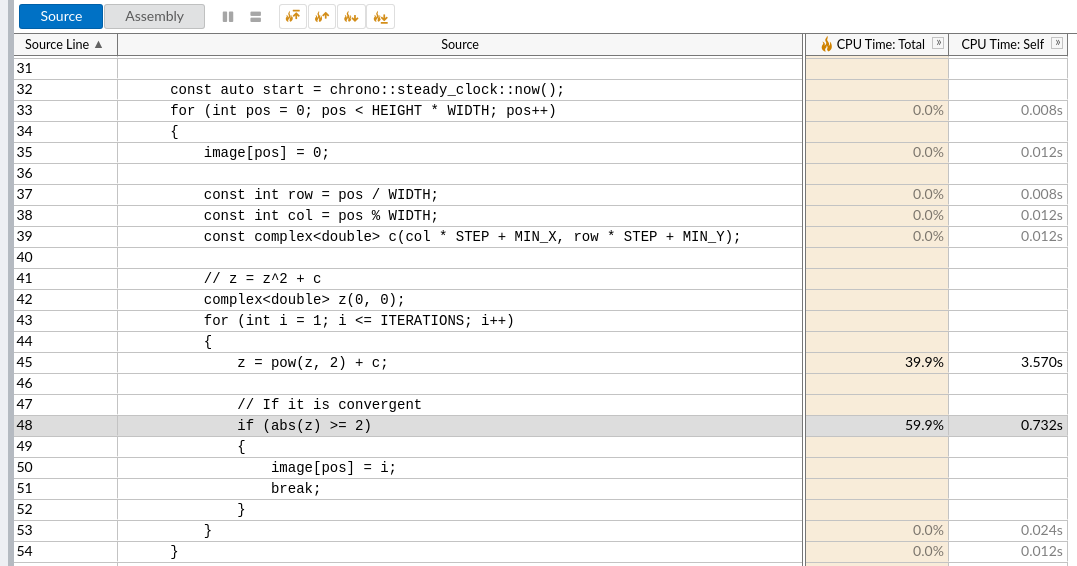
\includegraphics[width=0.8\textwidth]{assets/hotspots/hotspots.png}
\end{center}

\subsection{Conclusions}
The main hotspot is the DFT() function and its inverse IDFT(), which together account for over 99,05\% of the total execution time. All other functions have negligible impact. This indicates that \textbf{parallelization and vectorization efforts should focus on the double loop inside DFT()}.\\

\noindent
\textbf{The main hotspot is the loop contained in lines 72-80 (source: \texttt{src/omp\_homework.c})}. The dominant operations contributing to the algorithm's computational intensity are the \texttt{sin()} and \texttt{cos()} trigonometric functions, which account for the majority of the execution time, as shown in the following code.

\begin{figure}[ht]
    \centering
    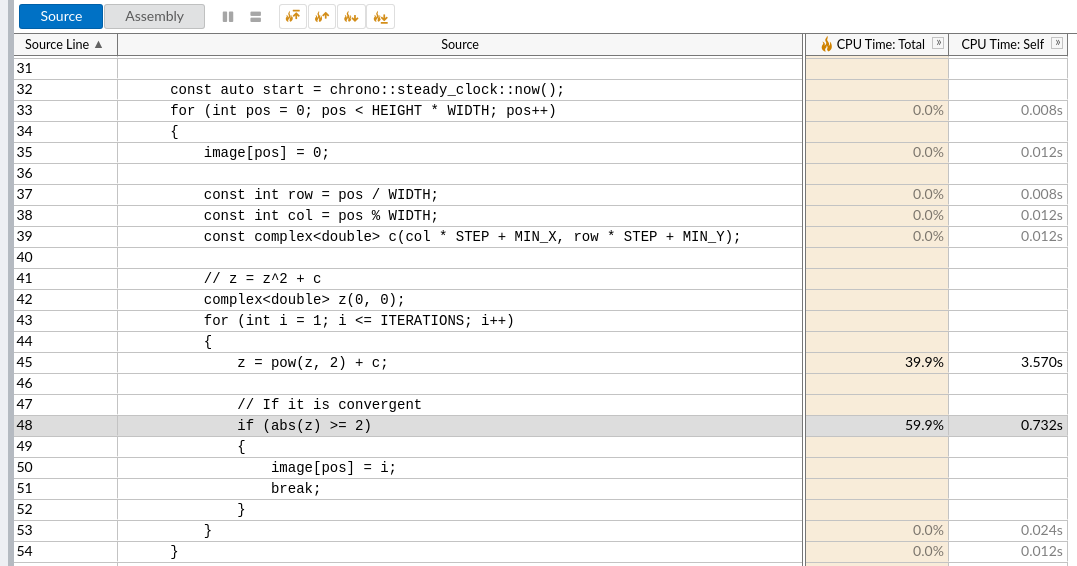
\includegraphics[width=0.9\textwidth]{assets/hotspots/hotspots.png}
    \label{fig:vtune_biggest_hotspot_screen}
\end{figure}
